\documentclass[11pt]{article}

%%
%% PACKAGES
%%

% Margins
\usepackage[margin=0.9in, top=0.8in, bottom=1.0in]{geometry}

% Fonts, typesetting, and math symbols
\usepackage[T1]{fontenc}
\usepackage{tgpagella} % Palatino-based font from TeX Gyre
\usepackage[scaled]{beramono} % Lovely monospace font
\usepackage{tgheros} % Helvetica-based font for headings
\usepackage{amsmath, amssymb}
\usepackage{mathtools}
\usepackage{mathdots}
\usepackage{microtype}
\usepackage{xspace}
\usepackage{xfrac}
\usepackage{calc}

% Plotting and drawing
\usepackage{tikz} % This automatically loads graphicx!
%\usetikzlibrary{calc} % For relative positions to defined coords
%\usepackage{pgfplots} % Scientific plotting tools
%\pgfplotsset{compat=1.7}

% Graphics
%\usepackage{graphicx}
%\usepackage[update,prepend]{epstopdf}
\usepackage{titlesec}
\usepackage{color}

% Table improvements
\usepackage{booktabs}

% Figure placement
%\usepackage{wrapfig}

% Code listings
\usepackage{listings}
\usepackage{matlab-prettifier}	% MATLAB code listings

% Tweaks for captions and enumerations
\usepackage[labelfont=bf]{caption}
%\captionsetup[wrapfigure]{margin=0.5cm}
\usepackage{enumitem}
\setlist[itemize]{itemsep=3pt,leftmargin=*,label=\textbullet}

% Fancy headers
\usepackage{fancyhdr}
\setlength{\headheight}{0pt}
\setlength{\footskip}{50pt}
\renewcommand{\headrulewidth}{0pt}
\renewcommand{\footrulewidth}{0pt}

%%
%% SETTINGS
%%

% Path to look for graphics
\graphicspath{{../images/}}

% Caption spacing
\setlength{\abovecaptionskip}{0pt}

% List spacing
\setlist{noitemsep}

% Table spacing
\renewcommand{\arraystretch}{1.3}

% Math operator font
% Note that cmr=roman and cmss=sans-serif.
\DeclareSymbolFont{sfoperators}{OT1}{cmr}{m}{n}
\DeclareSymbolFontAlphabet{\mathsf}{sfoperators}
\makeatletter
\def\operator@font{\mathgroup\symsfoperators}
\makeatother

%% No indent all paragraphs
%\setlength{\parindent}{0in}

% Figure and table references
\newcommand{\figref}[1]{Figure~\ref{#1}}
\newcommand{\tabref}[1]{Table~\ref{#1}}

% Special format section headings
\titleformat{\section}%
	{\color{blue}\large}% Text formatting
	{Part \arabic{section}}% Number
	{1em}% Space between number and text
	{}% Code before
	[\addvspace{-10pt}\rule{\textwidth}{0.4pt}]% Code after
\titleformat{\subsection}%
	{\color{blue}\normalsize\itshape}% Text formatting
	{Problem \arabic{section}.\arabic{subsection}}% Number
	{1em}% Space between number and text
	{}% Code before
	[\addvspace{-10pt}\rule{\widthof{Problem \arabic{section}.\arabic{subsection}}}{0.4pt}]% Code after
\titleformat{\subsubsection}%
	{\color{blue}}% Text formatting
	{\arabic{subsubsection} $\rightarrow$}% Number
	{1em}% Space between number and text
	{}% Code before
	[]% Code after

\definecolor{mygray}{rgb}{0.4, 0.4, 0.4}
\lstset{
style=Matlab-editor,
mlscaleinline=false,
basicstyle=\ttfamily\lst@ifdisplaystyle\scriptsize\fi,
frame=single,
rulecolor=\color{mygray},
numbers=left,
numbersep=10pt,
numberstyle=\footnotesize \ttfamily \color{mygray},
xleftmargin=30pt,
xrightmargin=5pt,
framexleftmargin=4pt,
framextopmargin=2pt
}

%%
%% COMMANDS
%%

% Draw legend lines for plots within the text. The \DeclareRobustCommand makes it work within figure captions.
\DeclareRobustCommand{\legendline}[1]{\raisebox{2pt}{\tikz{\draw[line width=2pt,#1](0,0) -- (5mm,0);}}}

% Superscript text: 1st, 2nd, 3rd, 4th
\newcommand{\suptext}[1]{\ensuremath{^\text{#1}}\xspace}
\newcommand{\st}{\suptext{st}}
\newcommand{\nd}{\suptext{nd}}
\newcommand{\rd}{\suptext{rd}}
\let\oldth\th % Reassign the current \th command
\renewcommand{\th}{\suptext{th}}

% Big O notation
\newcommand{\bigo}{\ensuremath{\mathcal{O}}}

% Fluid dynaimics terms
\newcommand{\ubar}{\ensuremath{\overline{u}}}
\newcommand{\Sbar}{\ensuremath{\overline{S}}}
\newcommand{\Wbar}{\ensuremath{\overline{W}}}

% Derivatives
\newcommand{\dd}[2]{\ensuremath{\frac{d #1}{d #2}}}
\newcommand{\pdd}[2]{\ensuremath{\frac{\partial #1}{\partial #2}}}
\newcommand{\tdd}[2]{\ensuremath{d #1 / d #2}}
\newcommand{\tpdd}[2]{\ensuremath{\partial #1 / \partial #2}}

% Bold vectors
\let\oldvec\vec
% Option 1: Works on more than single tokens, but makes regular letters italic as well as bold.
%\renewcommand{\vec}[1]{\mathbold{#1}}
% Option 2: Only works if a single token is passed to the command, but makes regular letters bold only.
\renewcommand{\vec}[1]{
	\ifcat\noexpand#1\relax
		\expandafter\mathbold
	\else
		\expandafter\mathbf
	\fi{{#1}}}

% Underlined vectors and double-underline matrices
\newcommand{\uvec}[1]{\ensuremath{\underline{#1}}}
\newcommand{\umat}[1]{\ensuremath{\underline{\underline{#1}}}}

% Engineering notation
\newcommand{\e}[1]{\ensuremath{\times 10^{#1}}}

% Expectation value and mean
\newcommand{\mean}[1]{\ensuremath{\overline{#1}}}
\newcommand{\expectation}[1]{\ensuremath{\left< #1 \right>}}
% Use the following inside text.
\newcommand{\texpectation}[1]{\ensuremath{\langle #1 \rangle}}

% Absolute value and norm bars
\DeclarePairedDelimiter\abs{\lvert}{\rvert}%
\DeclarePairedDelimiter\norm{\lVert}{\rVert}%
% Swap the definition of \abs* and \norm*, so that \abs
% and \norm resizes the size of the brackets, and the 
% starred version does not.
\makeatletter
\let\oldabs\abs
\def\abs{\@ifstar{\oldabs}{\oldabs*}}
\let\oldnorm\norm
\def\norm{\@ifstar{\oldnorm}{\oldnorm*}}
\makeatother

% Vertical asymptote for tikz/pgfplots
\newcommand{\vasymptote}[2][]{
    \draw [densely dashed,#1] ({rel axis cs:0,0} -| {axis cs:#2,0}) -- ({rel axis cs:0,1} -| {axis cs:#2,0});
}

% Vertical dirac delta function for tikz/pgfplots
\newcommand{\diracdelta}[2][]{
    \draw [#1] ({current axis.left of origin} -| {axis cs:#2,0}) -- ({rel axis cs:0,1} -| {axis cs:#2,0});
}

%%
%% DOCUMENT START
%%

\begin{document}

\pagestyle{fancyplain}
\lhead{}
\chead{}
\rhead{}
\lfoot{ASEN 6037: Project 2}
\cfoot{\thepage}
\rfoot{Ryan Skinner}

\noindent
{\Large \color{blue} Project 2}
\hfill
{\large Ryan Skinner}
\\[0.5ex]
{\large ASEN 6037: Turbulence}
\hfill
{\large Due 2015/05/08}
\hrule
\vspace{12pt}

In this project, we assess the strengths and shortcomings of Reynolds-averaged Navier-Stokes (RANS) models through derivations and comparison to DNS simulations of various flow classes.

\section{Derivation of RANS Models}

Please see the attached handwritten work; much of this problem consists of derivations which are long enough to preclude typesetting in a reasonable amount of time.

\section{Testing of RANS Models: Turbulent Channel Flow}

\subsection{}
%%
% Problem 2.1
%%

Consider a fully-developed turbulent channel flow. In such a flow, which of the components of $\ubar_i$, $\Sbar_{ij}$, and $\Wbar_{ij}$ are non-zero? What are $\tpdd{}{t}$ and $\ubar_i \tpdd{}{x_i}$? Comment on the validity of the equilibrium assumption used in Problem 1.8.

We will assume this turbulent channel flow to be either two- or three-dimensional, with the stream-wise direction denoted by $x$, and the span-wise direction(s) denoted by $y$.

Only $\ubar_x$ is non-zero, since this is the mean direction of flow. Any non-zero $\ubar_y$ would violate symmetry and, if near a wall, also the no-penetration boundary condition.

In the core flow away from the walls, all components of $\Sbar_{ij}$ are zero, since the velocity profile has negligible gradients in all directions ($\tpdd{}{x}$ is identically zero in a fully-developed flow). In the near-wall region, $\Sbar_{ij}$ does have non-zero components, because there is a large velocity gradient in the wall-normal direction. In this region, $\Sbar_{xy}$ is non-zero; it involves the derivative of the stream-wise velocity with respect to the wall-normal direction. All other components are zero because span-wise mean velocities are zero.

In a similar manner, all components of $\Wbar_{ij}$ are zero in the core flow. Again, this is because there exist no substantial velocity gradients in the core region. In the near-wall region, however, hairpin vortices peel off and create preferential vorticity. These structures create zero mean downstream and wall-normal vorticity due to symmetry of the hairpin, but non-zero vorticity in the direction of $(\text{wall-normal} \times \text{stream-wise})$. Taking the channel to be three-dimensional, if we consider the flow direction to be into the page $x$, along the bottom wall (whose normal is in the $y$-direction, pointing into the channel) vorticity will be preferentially in the $-\hat{z}$-direction. Thus, near this wall, $\Wbar_{xy}$ and $\Wbar_{yx}$ will be non-zero. Similar arguments apply to the other walls.

Since the flow is fully-developed, the averages of flow quantities will have no change in time, making $\tpdd{}{t}=0$. However, there will still be fluctuations in the flow for which $\tpdd{}{t} \neq 0$. For the convective derivative, we already know that spatial derivatives in the stream-wise direction must be zero, so $\ubar_x \tpdd{}{x}=0$. Additionally, there are no mean velocities in the span-wise directions, so $\ubar_y=0$. Thus all $\ubar_i \tpdd{}{x_i}=0$.

In conclusion, the equilibrium assumption that postulates constant anisotropy is an acceptable one for average quantities. Though this is not true for fluctuating, instantaneous quantities, we will presumably be using the RANS equations for modelling, in which only average quantities are used.

\subsection{}
%%
% Problem 2.2
%%

Using the turbulent channel flow DNS data from Moser, Kim, and Mansour (1999), we calculate and plot the non-zero components of $\ubar_i$, $\overline{u'_i u'_j}$, $k$, $\epsilon$, $a_{ij}$, and $\Sbar_{ij}$ as functions of both $y^+$ and $y/h$. Results are displayed in \figref{fig:part2_ubar} through \figref{fig:part2_Sij}

\begin{figure}[p]
\centering
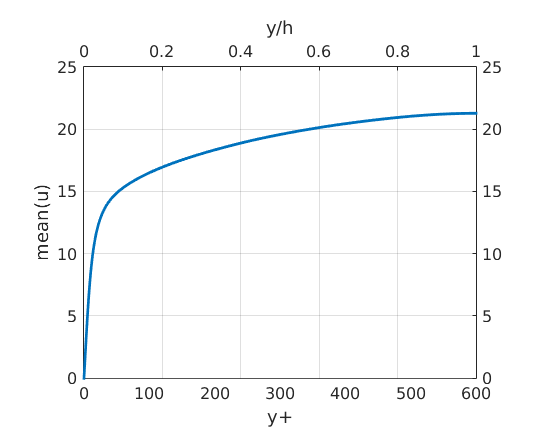
\includegraphics[scale=0.85]{part2_ubar.png}
\vspace{6pt}
\caption{Mean velocity in the stream-wise direction.}
\label{fig:part2_ubar}
\end{figure}

\begin{figure}[p]
\centering
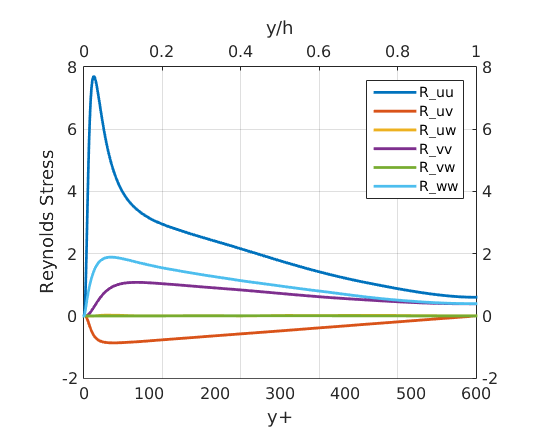
\includegraphics[scale=0.85]{part2_reystress.png}
\vspace{6pt}
\caption{Components of the Reynolds stress tensor.}
\label{fig:part2_reystress}
\end{figure}

\begin{figure}[p]
\centering
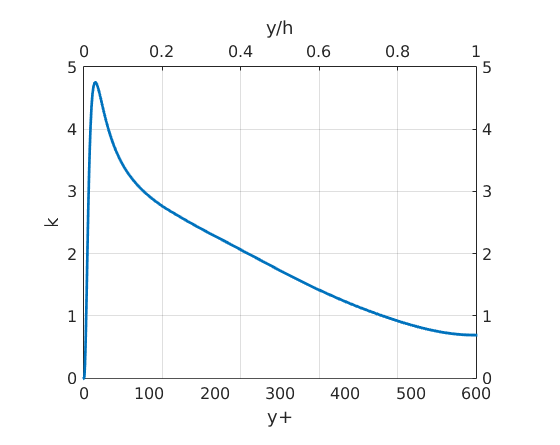
\includegraphics[scale=0.85]{part2_k.png}
\vspace{6pt}
\caption{Turbulence intensity.}
\label{fig:part2_k}
\end{figure}

\begin{figure}[p]
\centering
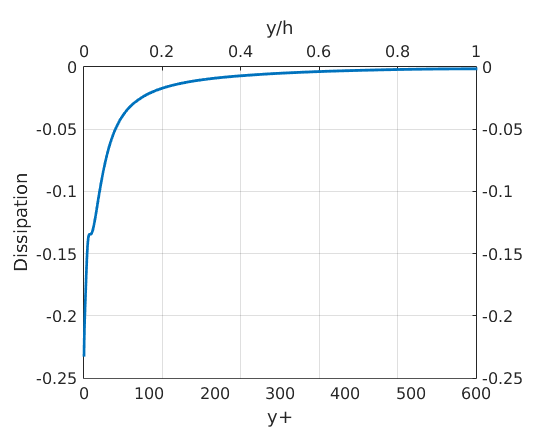
\includegraphics[scale=0.85]{part2_epsilon.png}
\vspace{6pt}
\caption{Turbulent kinetic energy dissipation.}
\label{fig:part2_epsilon}
\end{figure}

\begin{figure}[p]
\centering
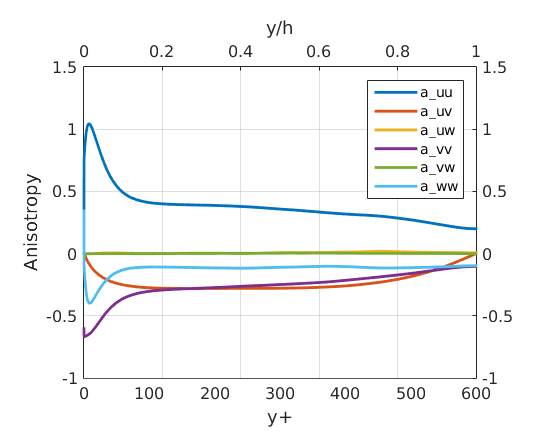
\includegraphics[scale=0.85]{part2_aij.png}
\vspace{6pt}
\caption{Components of the anisotropy tensor.}
\label{fig:part2_aij}
\end{figure}

\begin{figure}[p]
\centering
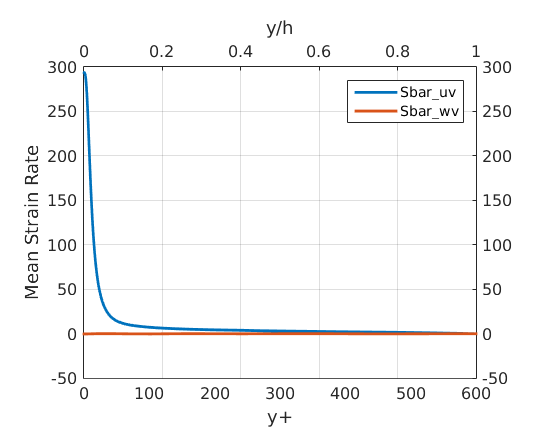
\includegraphics[scale=0.85]{part2_Sij.png}
\vspace{6pt}
\caption{Components of the mean strain rate tensor; all components not shown are zero. Additionally, $\Sbar_{wv}$ should be zero in an ideal flow because there should be no mean span-wise velocities.}
\label{fig:part2_Sij}
\end{figure}

\subsection{}
%%
% Problem 2.3
%%

Using $a_{12}$ and $\Sbar_{12}$, the mean value of the eddy viscosity coefficient $C_\mu$ away from the walls ($y/h > 0.2$) is calculated to be approximately 0.086. This is the constant value that gives the closest agreement between the computational data and the closure model of
\begin{equation}
C_\mu =
\frac{-\epsilon a_{12}}{2k \Sbar_{12}}
.
\end{equation}
A plot of $C_\mu$ and its average value away from the wall is presented in \figref{fig:part2_Cmu}.

\begin{figure}[p]
\centering
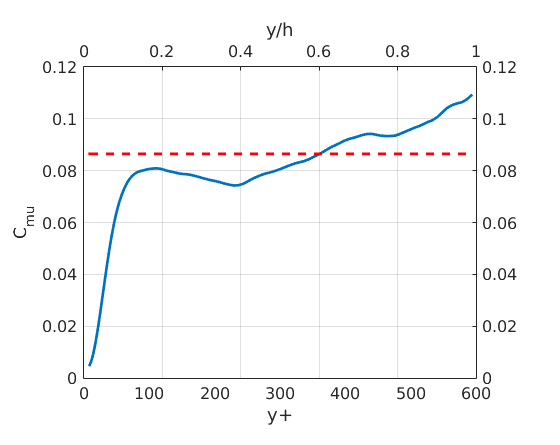
\includegraphics[scale=0.85]{part2_Cmu.png}
\vspace{6pt}
\caption{Eddy viscosity coefficient $C_\mu$ as a function of distance from wall, calculated using $a_{12}$ and $\Sbar_{12}$. The average value is 0.086 for $y/h > 0.2$.}
\label{fig:part2_Cmu}
\end{figure}

\subsection{}
%%
% Problem 2.4
%%

The closure from problem 1.9,
\begin{equation}
a_{ij} =
-2 \frac{\nu_T}{k} \Sbar_{ij}
,
\qquad
\text{where}
\qquad
\nu_T =
C_\mu \frac{k^2}{\epsilon}
,
\label{eq:14}
\end{equation}
fails to capture important physical effects near the channel walls. $C_\mu$ should drop significantly in the near-wall region, for roughly $y^+ < 75$, but it does not. This failure occurs for at least two reasons.

First, the gradient transport hypothesis that was used to derive \eqref{eq:14} only holds (if at all) away from the walls. Near the walls, velocities and Reynolds numbers decrease to the point where viscous diffusion plays a large role in the flow dynamics. The gradient transport hypothesis assumes that $Re_\tau$ is high, and that transport within the flow is almost exclusively due to small eddies, rather than large eddies or viscous effects.

Second, we recall from Problem 1.8 that the equilibrium assumption led to the $a_ij$ closure of \eqref{eq:14}, which yielded
\begin{equation}
a_{ij} =
\frac{\alpha_2}{\alpha_1} \frac{k}{\epsilon} \Sbar_{ij} =
\frac{C2-(4/3)}{(P/\epsilon)-1+C_1} \frac{k}{\epsilon} \Sbar_{ij}
.
\end{equation}
Of note here is that the production term $P$ was neglected when deriving \eqref{eq:14}. Turbulence production is important near the boundaries because of the high mean shear, and it is absent from \eqref{eq:14}.

\subsection{}
%%
% Problem 2.5
%%

A popular approach to improving the closure from \eqref{eq:14} near channel walls is to limit $C_\mu$ such that
\begin{equation}
C_\mu =
\begin{cases}
0.09 &\text{for $(Sk/\epsilon) \le 3.4$} \\
0.31(Sk/\epsilon)^{-1} &\text{for $(Sk/\epsilon) > 3.4$}
\end{cases}
\end{equation}

This has a positive effect on the model near channel walls. As one approaches the wall, the relative shear strength $(Sk/\epsilon)$ increases dramatically, and this method allows $C_\mu$ to drop continuously from its limit of 0.09 to much smaller values near the wall, inversely proportional to the relative shear strength. According to \figref{fig:part2_Sij}, the strain rate really starts to pick up approaching the wall around $y^+ \approx 50$, and this is roughly where $C_\mu$ would need to start dropping to account for wall effects as seen in \figref{fig:part2_Cmu}.

I would consider this a decent approach to correcting our turbulence model in the near-wall region. It is a model and thus will not be perfect, but it seems to respond to the wall in a physically-justified fashion at the appropriate distance. This presumes that the activation value of $(Sk/\epsilon) = 3.4$ has been chosen in good agreement with empirical data. It is also convenient that the cut-off model for $C_\mu$ is easily computed.

\subsection{}
%%
% Problem 2.6
%%

From a physical perspective, turbulence models have difficulty for $y^+ < 30$ for a number of reasons. First, in deriving models we often make high-$Re$ assumptions that are invalid near the wall. This leads to a neglect of viscous effects as well as anisotropy and turbulence kinetic energy production due to shearing. It is also common to assume that $\epsilon_{ij}$ is isotropic, as noted in Problem 1.5 due to K41 theory, but this too breaks down near the walls. This becomes particularly problematic when these anisotropic turbulent structures form near the walls and are convected into the core flow.

Very close to the walls, the log law,
\begin{equation}
y^+ =
\frac{1}{\kappa} \ln y^+ + B
,
\end{equation}
constitutes a better mathematical function that allows for more accurate prediction of $a_{ij}$. For \emph{very} near-wall physics, the viscous sublayer relationship of $u^+ = y^+$ would be the most accurate.

\subsection{}
%%
% Problem 2.7
%%

If we write $a_{ij}$ using its modelled form from \eqref{eq:14}, we can substitute it into the equation for the Reynolds stresses, yielding, after some simplification,
\begin{equation}
\overline{{u'_\alpha}^2} =
\frac{2}{3}k
\left(
1 - C_\mu \frac{k}{\epsilon} \Sbar_{\alpha \alpha}
\right)
,
\end{equation}
where no summation is implied over Greek indices by convention. However, note that $\Sbar_{\alpha\alpha}$ involves derivatives of mean flow velocities in the same spatial direction. In this flow, mean span-wise velocities are zero, and flow statistics are invariant in the stream-wise direction. Thus $\Sbar_{\alpha\alpha} = 0$ and we are left with the isotropic form
\begin{equation}
\overline{{u'_i}^2} = \frac{2}{3} k
.
\end{equation}

Referencing \figref{fig:part2_reystress}, the diagonal Reynolds stresses are very much \emph{not constant} in the DNS flow, nor are they equal to one another. The only saving grace of our model is that both it and the DNS results show diagonal Reynolds stresses summing to double the turbulence intensity $k$, but this occurs by definition.

The discrepancies can be explained as follows. First, we dropped all redistribution terms very early on in the derivation of our model. This makes it impossible for anisotropy to move between different components of $a_{ij}$ as fluid parcels are subjected to convection and shear. Additionally, the gradient transport hypothesis we employed assumed that small scale eddies were solely responsible for transport phenomena. Because we dictated that $\epsilon_{ij}$ be isotropic from K41, it comes as little surprise that giving sole dynamic importance to these isotropic small scales results in an isotropic flow at all scales.

\subsection{}
%%
% Problem 2.8
%%

In conclusion, this closure model is simple and easy to implement, but inaccurate for wall-bounded flows, especially in the near-wall region. Even in the core flow regions, assuming a constant $C_\mu$ is not particularly accurate, as can be seen in \figref{fig:part2_Cmu}. This leads to inaccuracies when simulating flows with small-scale production, such as combustion or wind moving through trees. As we determined by looking at the model's treatment of diagonal Reynolds stresses, flows with any degree of anisotropy will be poorly-represented with this closure model. Having assumed equilibrium, unsteadiness in flows will also be ill-resolved. Idealized flows without boundary layers, without time-varying phenomena, and without any appreciable degree of anisotropy will be resolved fairly well with this turbulence model.

Most real-world engineering flows fall into these categories, which makes it surprising that such a model so so widely-employed in industry. Nonetheless, the simplicity and speed with which the governing equations can be numerically solved is appealing in a production environment. Presumably, these types of models assist with rapid iteration of design. Despite it's shortcomings, this model is probably `good enough' to reach a decent design that can be refined using more experienced humans or higher-fidelity models.

\section{Testing of RANS Models: Unsteady Homogeneous Flow}

Problems 3.1--3.4 consist mostly of derivations which are not typeset here, but are included in the attached handwritten documents.
\setcounter{subsection}{4}

\subsection{}
%%
% Problem 3.5
%%

Assuming that $a_{12}=0$ at $t=0$, we numerically integrate the set of ordinary differential equations found in Problem 3.4 for the SKE and DKE models. We take $S^* \equiv S k_0 / \epsilon_0 = 3.3$, and examine the flow evolution for $(\omega/S) = \{0.01,0.1,0.5,1,10\}$. The evolution of $a_{12}$ is plotted as a function of $S \cdot t = S^* \tau$ for each of the $\omega/S$ values and both models. We furthermore assume that $C_\mu = 0.09$ in the SKE model.

\subsection{}
%%
% Problem 3.6
%%

\subsection{}
%%
% Problem 3.7
%%

\section{Testing of RANS Models: Computational Fluid Dynamics Code}

\subsection{}
%%
% Problem 4.1
%%

%%
%% DOCUMENT END
%%
\end{document}












